\section{Internal Combustion Engine Simulator}
%
ICESym es un simulador de motores de combustión interna que  utiliza modelos 0D
para la cámara de combustión y 1D para el flujo a través del sistema de
intercambio de gases.
%
Permite evaluar la \emph{performance} de un motor a un costo computacional bajo
además, la implementación de entrada y salida de datos permite utilizar el
simulador como una \emph{caja negra} de modo que se pudo implementar en un
\emph{script} como una función a la que se le otorga un conjunto de parámetros
de entrada y devuelve los resultados de la simulación en un formato que permite
la lectura y evaluación de los mismos.
%
Contiene en su código las rutinas necesarias para simular el ciclo operativo y la
geometría del MRCVC.

Se realizaron modificaciones menores al simulador para facilitar la ejecución en
conjunto con el optimizador, algunas de estas modificaicones fueron:
%
\begin{enumerate}
    \item Modificar los archivos de salida, eliminando valroes que no se
utilizaron, de modo de reducir el tamaño de los archivos de salida, facilitar la
lectura y el procesamiento de datos.
    \item Incluir una opción para elegir entre un modelo de $C_D$ de una o dos
variables.
    \item Modificar el área de referencia.
    \item Agregar una interpolación bilineal para podes trabajar con el mapa de
$C_D$.
\end{enumerate}


\section{Modificaciones a ICESym}
%%%%%%%%%%%%%%%%%%%%%%%%%%%%%%%%%%%%%%%%%%%%%%%%%%%%%%%%%%%%%%%%%%%%%%%%%%%%%%%
\subsection{Flujo a través de los puertos}
%
Para tener un mejor modelado del flujo de gas a través de los puertos de
admisión y escape, se introdujo una opción para poder ejecutar ICESym con un
modelo del coeficiente de descarga que dependa de dos variables, diferencia de
presión y \emph{alzada} o apertura del puerto $C_D = f(\Delta P; lv)$.
%
Esto significó agregar una opción que permita seleccionar entre un $C_D$ que
depende únicamente de una o dos variables.

Con esto se construye una mapa del coeficiente de descarga de la forma $C_D =
f(lv, dp)$, que se utiliza para calcular el área efectiva de la válvula.

Independientemente de la cantidad de variables que formen parte del $C_{D}$, a
ICESym se introduce un vector o matriz para el caso 1D o 2D respectivamente.
%
En ambos casos se intrudce una cantidad discreta de valores por lo que es
necesario realizar una interpolación lineal o bilineal para utilizar el valor de
$C_{D}$ correspondiente a un valor de $l_{v}$ o par $(l_{v}, \Delta_{P})$.
%
La interpolación lineal 1D es parte del código de ICESym, la interpolación 2D o
bilineal se introdujo como parte de este trabajo.

Esta última se realiza sobre una malla rectangular, de modo de reutilizar el
código existente de para el caso 1D y realizar  simplemente una interpolación
lineal entre dos valores en planos con datos conocidos.

En la rutina de Fortran que sigue, se describe la interpolación 1D comentada del
código de ICESym.

\begin{lstlisting}[basicstyle=\scriptsize, language=fortran, caption=Interpolación 1D]
SUBROUTINE interpolant(x, y, xi, yi)
   ! x: vector con valores conocidos de x ordenados de menor a mayor
   ! y=f(x)
   ! xi: valor de x para el que se quiere conocer yi=f(xi)
   IMPLICIT NONE
   REAL*8, INTENT(in) :: xi
   REAL*8, DIMENSION(:), INTENT(in) :: x, y
   REAL*8, INTENT(out) :: yi
   ! nx: es la cantidad de elementos en x
   ! i: es un entero que se usa en la rutina
   INTEGER :: nx, i
   nx = SIZE(x)
   ! Si xi es menor al primer elemento del vector x, a yi se le
   ! asigna el primer valor del vector y, saliendo de la rutina
   IF (xi .LT. x(1)) THEN
      yi = y(1)
      RETURN
   END IF
   ! Si xi es mayor que el último elemento del vector x, a yi se le
   ! asigna el último valor del vector y, saliendo de la rutina
   IF (xi .GT. x(nx)) THEN
      yi = y(nx)
      RETURN
   END IF
   ! iminloc busca el índice del elemento de x, x(i) que está más cercano a
   ! xi.
   ! dabs es una subrutina que devuelve el valor absoluto
   i = iminloc(dabs(x - xi))
   ! Si algún valor de x coincide con xi, a yi se le asigna el valor de
   ! y=f(x(i)), saliendo de la rutina
   IF (x(i) .EQ. xi) THEN
      yi = y(i)
      RETURN
   END IF
   ! Si x(i) es mayor a xi, se utiliza el valor anterior x(i-1) para la
   ! interpoación
   IF (x(i) .GT. xi) i = i - 1
   ! Se procede a interpolar el valor y=f(xi) y se sale de la rutina
   yi = y(i) + (xi - x(i))*(y(i + 1) - y(i))/(x(i + 1) - x(i))
END SUBROUTINE interpolant
\end{lstlisting}


La interpolación 2D utiliza la interpoación 1D
\begin{lstlisting}[basicstyle=\scriptsize, language=fortran, caption=Interpolación 2D]
SUBROUTINE interpolant2d(x, y, z, xi, yi, zi)
   ! x: vector con valores conocidos de x ordenados de menor a mayor
   ! y: vector con valores conocidos de y ordenados de menor a mayor
   ! z=f(x, y)
   ! xi, yi: par de (x,y) para el que se quiere conocer zi=f(xi, yi)
   ! zi: valor de salida
   IMPLICIT NONE
   REAL*8, DIMENSION(:), INTENT(in) :: x, y
   REAL*8, DIMENSION(:, :), INTENT(in) :: z
   REAL*8, INTENT(in) :: xi, yi
   REAL*8, INTENT(out) :: zi
   INTEGER :: nx, i
   REAL*8, DIMENSION(2) :: z_aux

   nx = SIZE(x)
   IF (xi .LE. x(1)) THEN ! <=
      CALL interpolant(y, z(1, :), yi, zi)
      RETURN
   ELSE IF (xi .GE. x(nx)) THEN  ! >=
      CALL interpolant(y, z(nx, :), yi, zi)
      RETURN
   END IF

   i = iminloc(dabs(x - xi))
   IF (x(i) .GT. xi) i = i - 1 ! >

   CALL interpolant(y, z(i, :), yi, z_aux(1))   ! z1=f(x1,yi)
   CALL interpolant(y, z(i + 1, :), yi, z_aux(2)) ! z2=f(x2,yi)
   CALL interpolant(x(i:i + 1), z_aux, xi, zi)   ! zi=f(xi,yi)

END SUBROUTINE interpolant2d
\end{lstlisting}

% \begin{algorithm}
%   \SetAlgolined
%   \KwIn{(x, y, z): puntos conocidos.\\
%     $(x_{i}, y_{I})$: puntos donde se quiere conocer $z_{i}$.\\
%     INTERPOLANT: función de interpolación en una dimensión.\\
%   }
%   \KwResult{$z_{i}$ valor de z buscado para el par $(x_{i}, y_{i})$.}
%   $n$ \LeftArrow es la cantidad de elementos de x
%   \eIf{
%     $x_{i} \geq x_{n}$
%   }{
%     $z_{i} \Leftarrow$ INTERPOLANT
%   }


% \begin{algorithm}
%  \caption{Interpolación bi-lineal}\label{algo:bilineal}
%     \SetAlgoLined
%     \SetKwFunction{Size}{Size}
%     \SetKwFunction{Interpolant}{Interpolant}

%     \KwIn{\\
%         $\vec{x}, \vec{y}$: valores de $x, y$ en los que se conoce el valor en $z$.\\
%         $\vec{z}$: valores conocidos de $z$.\\
%         $x_i, y_i$: puntos para realizar la interpolación.\\
%         INTERPOLANT: inerpolación 1D.\\
%       }
%     \KwResult{Devuelve el valor interpolado de $z_i$.}
%     $n_x \Leftarrow tamaño(x)$\;
%     \eIf{
%       $x_i \geq x_{n_x}$
%     }{
%       $z_i \Leftarrow INTERPOLANT(y, z[1,:], y_i)$\;
%       \Return\;
%     }{
%       $z_i \Leftarrow INTERPOLANT(y, z[n_x,:], y_i)$\;
%       \Return\;
%     }
%     $i \Leftarrow iminloc(dabas(x-x_i))$\;
% \end{algorithm}

Si bien hay otros métodos para estimar el valor de $C_D$ para dos valores $(\Delta
P; l_v)$, este método es sencillo y da resultados satisfactorios.
%
En la figura~\ref{fig:bilineal} se muestra un ejemplo del error obtenido con
este método para interpolar una función de prueba $\sin\left(\sqrt(x^2 + y^2)\right)$.

\begin{figure}
    \centering
    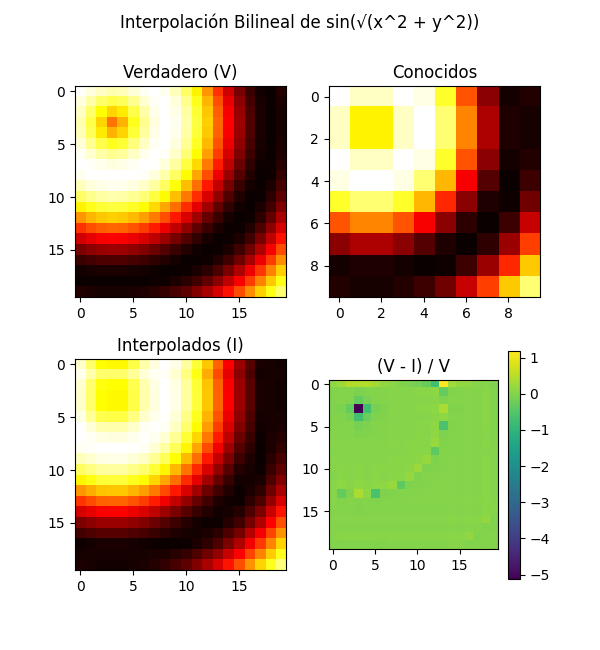
\includegraphics[width=0.7\textwidth]{bilineal.png}
    \caption{Interpolación bilineal de $\sin(\sqrt(x^2 + y^2))$}\label{fig:bilineal}
\end{figure}

La malla rectangular requerida para la interpolación bilineal del mapa de
$C_{D}$ se realizará a partir de los valores conocidos de $C_D$ resultantes de
las flujometrías con \emph{OpenFOAM}~\parencite{openfoam}.
%
Debido al costo computacional que requieren la flujometría, solo una cantidad
reducida de puntos se obtendrá con este método, esto  significa que se tiene
como punto de partida una malla no rectangular por lo que se utiliza un método
intermedio para obtener una matriz de puntos que pueda ser leído por la
interpolación bilineal.

Se probaron dos métodos para realizar la interpolación, el método del punto más
cercano y la interpolación por la suma de la inversa de la distancia o IDW por
sus siglas en inglés (\emph{Inverse Distance Weighting}).
%
Estos se combinan métodos de con suavizados de promedio móvil con los $n$
valores más cercanos.

El método del punto más cercano consiste en asignar para cada par $(x, y)$ el
valor conocido más cercano, el algoritmo es como se indica a continuación:

\begin{algorithm}
 \caption{Interpolación por punto más cercano}\label{algo:mas_cercano}
    \KwIn{\\
        $V_x, V_y$: valores de $x, y$ en los que se conoce el valor en $z$.\\
        $V_z$: valores conocidos de $z$.\\
        $I_x$: $n$ puntos de $x$ donde se quiere interpolar\\
        $I_Y$: $m$ puntos de $y$ donde se quiere interpolar\\
        }

    \KwResult{Devuelve una matriz $I_{[n,m]}$ con los valores interpolados,
      donde cada punto $I(x,y)$ se le asigna al valor de $V_Z$ más cercano
      conocido. Da como resultado superficies escalonadas.}

    \BlankLine
     $I=zeros_{[n,m]}$\;
     \For{$i \gets 0$\KwTo$n$}{
        \For{$j \gets 0$\KwTo$m$}{
          $d = \sqrt{{(V_x - I_{xi})}^2 + {(V_y - I_{yj})}^2}$\;
            $I[i,j] = v_z[\min(d)]$\;
        }
     }
\end{algorithm}

La interpolación IDW consiste en asignar a cada punto el resultado de un
promedio de los valores cercanos al punto en cuestión, ponderado por la
distancia al valor elevado a un exponente arbitrario $p$.
%
Cuanto mayor sea el valor de $p$, más sensible es el método a los valores
cercanos, la formulación de este método se ve en la ecuación~\ref{eq:idw} y la
algoritmo utilizado para calcular esto se detalla en~\ref{algo:IDW}
%
En la figura~\ref{fig:mapas_interpolados} se muestra una comparación de ambos
métodos, para una malla de $C_{D}=f(\Delta_{P}, l_{v})$ generada al azar.


\begin{equation} \label{eq:idw}
    f_p = \frac{\sum_{i=1}^{n} \frac{z_i}{d_i^p}} {\sum_{i=1}^{n}
    \frac{1}{d_i^p}}
\end{equation}


\begin{algorithm}
    \caption{Interpolación IDW}\label{algo:IDW}
    \KwIn{\\
        $V_x, V_y$: valores de $x, y$ en los que se conoce el valor en $z$.\\
        $V_z$: valores conocidos de $z$.\\
        $I_x$: $n$ puntos de $x$ donde se quiere interpolar\\
        $I_Y$: $m$ puntos de $y$ donde se quiere interpolar\\
        $p$: potencia a la que se eleva cada peso\\
        }

    \KwResult{Interpolación ponderada por inverso de la distancia. Dependiendo
      del valor de p, se obtienen valores más o menos suavizados.}

    \BlankLine
    $I=zeros_{[n,m]}$\;
    \For{$i \gets 0$\KwTo$n$}{
        \For{$j$\gets 0 \KwTo$m$}{
          $d = {\left[{(V_x - I_{xi})}^2 +{(V_y - I_{yj})}^2\right]}^{\frac{p}{2}}$\;
          \eIf{$\exists i : d[i] = 0$}{
            $I[i, j] = V_z[i]$\;
          }{
            $I[i,j] = \frac{\sum{V_{zi}/d_i}}{\sum \frac{1}{d}}$\;
          }
        }
     }
\end{algorithm}

\begin{figure}
    \centering
    \begin{subfigure}{0.4\textwidth}
        \centering
        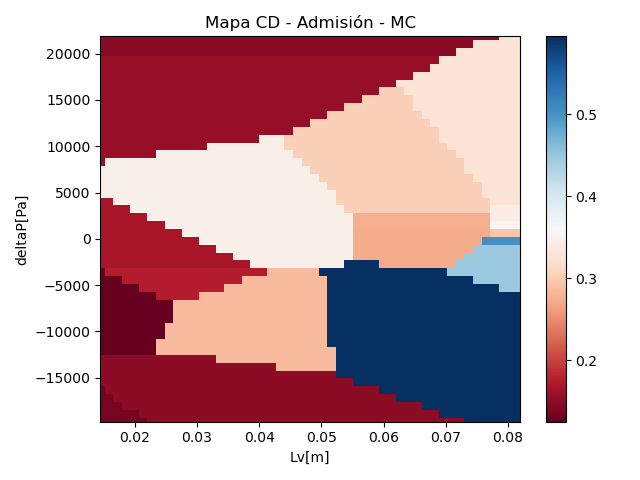
\includegraphics[width=\textwidth]{mapa_cd/mc_mapa_adm.png}
        \caption{Punto Más Cercano sin suavizar}
    \end{subfigure}
    \hfill
    \begin{subfigure}{0.4\textwidth}
        \centering
        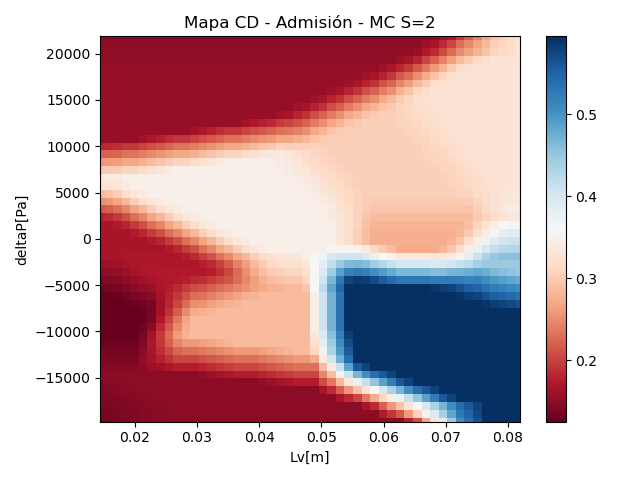
\includegraphics[width=\textwidth]{mapa_cd/mc_s2_mapa_adm.png}
        \caption{Más Cercano ($S=2$)}
    \end{subfigure}
    \hfill
    \begin{subfigure}{0.4\textwidth}
        \centering
        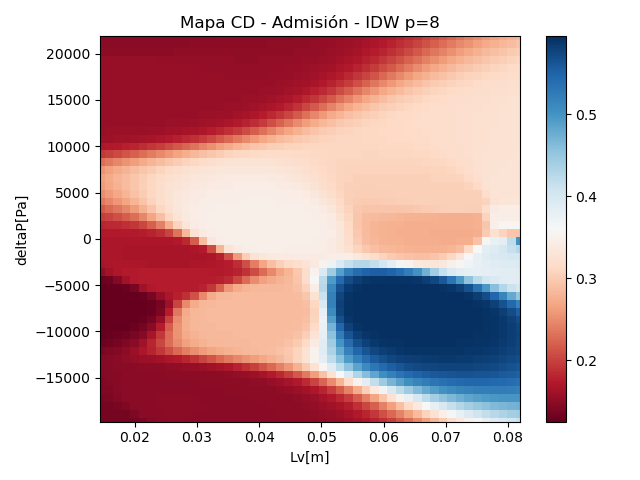
\includegraphics[width=\textwidth]{mapa_cd/idw8_mapa_adm.png}
        \caption{IDW ($p=8$)}
    \end{subfigure}
    \hfill
    \begin{subfigure}{0.4\textwidth}
        \centering
        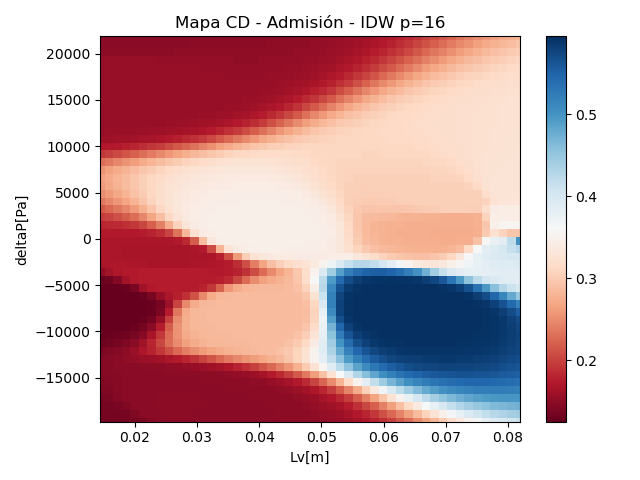
\includegraphics[width=\textwidth]{mapa_cd/idw16_mapa_adm.png}
        \caption{IDW ($p=16$)}
    \end{subfigure}
    \caption{Comparación de interpolaciones}\label{fig:mapas_interpolados}
\end{figure}

%%%%%%%%%%%%%%%%%%%%%%%%%%%%%%%%%%%%%%%%%%%%%%%%%%%%%%%%%%%%%%%%%%%%%%%%%%%%%%%

\subsection{Área de referencia}
%
El área de referencia utilizada por ICESym ese el área de
cortina~\ref{eq:area_cortina} y se expresa en el código del programa como el
área efectiva $F_{V}=A_{R}\cdot C_{D}$.
%
Cómo se indico en el apartado~\ref{sec:cap2_cd}, para el  MRCVC el área de
referencia es el área frontal del puerto expuesta a la cámara, calculada como la
altura de la ranura $h_{p}=\lua{tex.print{myData.hp}}\text{ mm}$ multiplicada
por la distancia entre el borde del puerto y la paleta que delimita la cámara,
denominado como $l_{v}$,

%
% En la figura~\ref{fig:area_referencia} se ilustran las áreas de referencia para
% una posición del rotor en la que hay solape de cámaras con $\theta = 55^\circ$.
%
Este valor se afecta por el coeficiente de descarga intermedio $C_{D,int}$, que
puede ser un valor fijo o el resultado de interpolar de un mapa de $C_D$ para un
valor de cuerda y $\Delta_P$ dado, ver~\ref{eq:fv}.

\begin{equation}\label{eq:fv}
    F_v = C_{D,int}\cdot 0.0294\cdot l_{v}
\end{equation}

% \begin{figure}
%     \centering
%     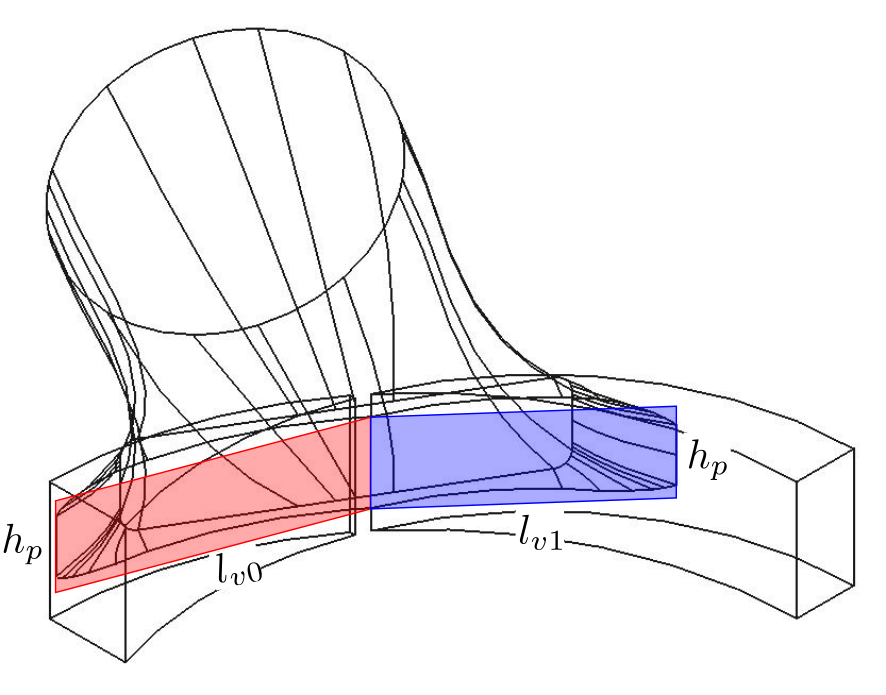
\includegraphics[]{area_referencia.png}
%     \caption{Área de referencia}\label{fig:area_referencia}
% \end{figure}

Tanto al inicio como al cierre del puerto ocurre solape de cámaras, por lo que
en estos intervalos angulares hay un valor de $C_D$ para cada cámara.
%
Este se calcula con el flujo másico que atraviesa los parches correspondientes
a cada cámara y el área de puerto expuesta por cada cámara.
% TODO: ver nota 8

\subsection{Interfaz con optimizador}
%
Para lograr ejecutar el simulador automáticamente, se hizo una librería de
funciones capaz de tomar como dato de entrada un archivo de configuración que
incluye geometría, velocidades a ejecutar y cantidad de ciclos de simulación
entre otros.

Para ejecutar una instancia de ICESym se puede utilizar la interfaz gráfica de usuario ó la interfaz de línea de comando.



Puesto que se utiliza el programa desarrollado para este trabajo y la simulación
se realiza de manera automática aprovechando la cualidad de ``caja negra'' de
ICESym y se utiliza la interfaz de línea de comandos.
%
El simulador se ejecuta como un archivo de Python ``>> python main.py'', este
archivo contiene las instrucciones que lanzan la simulación del motor con
una configuración dada.
%

Esto permite ejecutar la simuaclión de manera automatizada ya que el comando
para ejecutar el simulador se puede lanzar desde otro programa de python con
permisos para ejecutar comandos dentro de una consola de (en este caso) Linux.

(NOTA: preguntar si hace falta que ponga estos detalles? o está de más)
